
Because the Wt process produces events with a different extra jet spectrum from
\ttbar\, uncertainties on the Wt rate can be a source of systematic uncertainty
on the unfolding.  This uncertainty is studied using the baseline unfolding procedure
but varying the Wt contribution to the input spectrum between 0\%\ anf 5\%.
The results of this study are presented in Figure~\ref{fig:WtRat}.  The
resulting systematic uncertainy is at the sub-percent level.

\begin{figure}
\centering
\begin{subfigure}[]{0.3\textwidth}
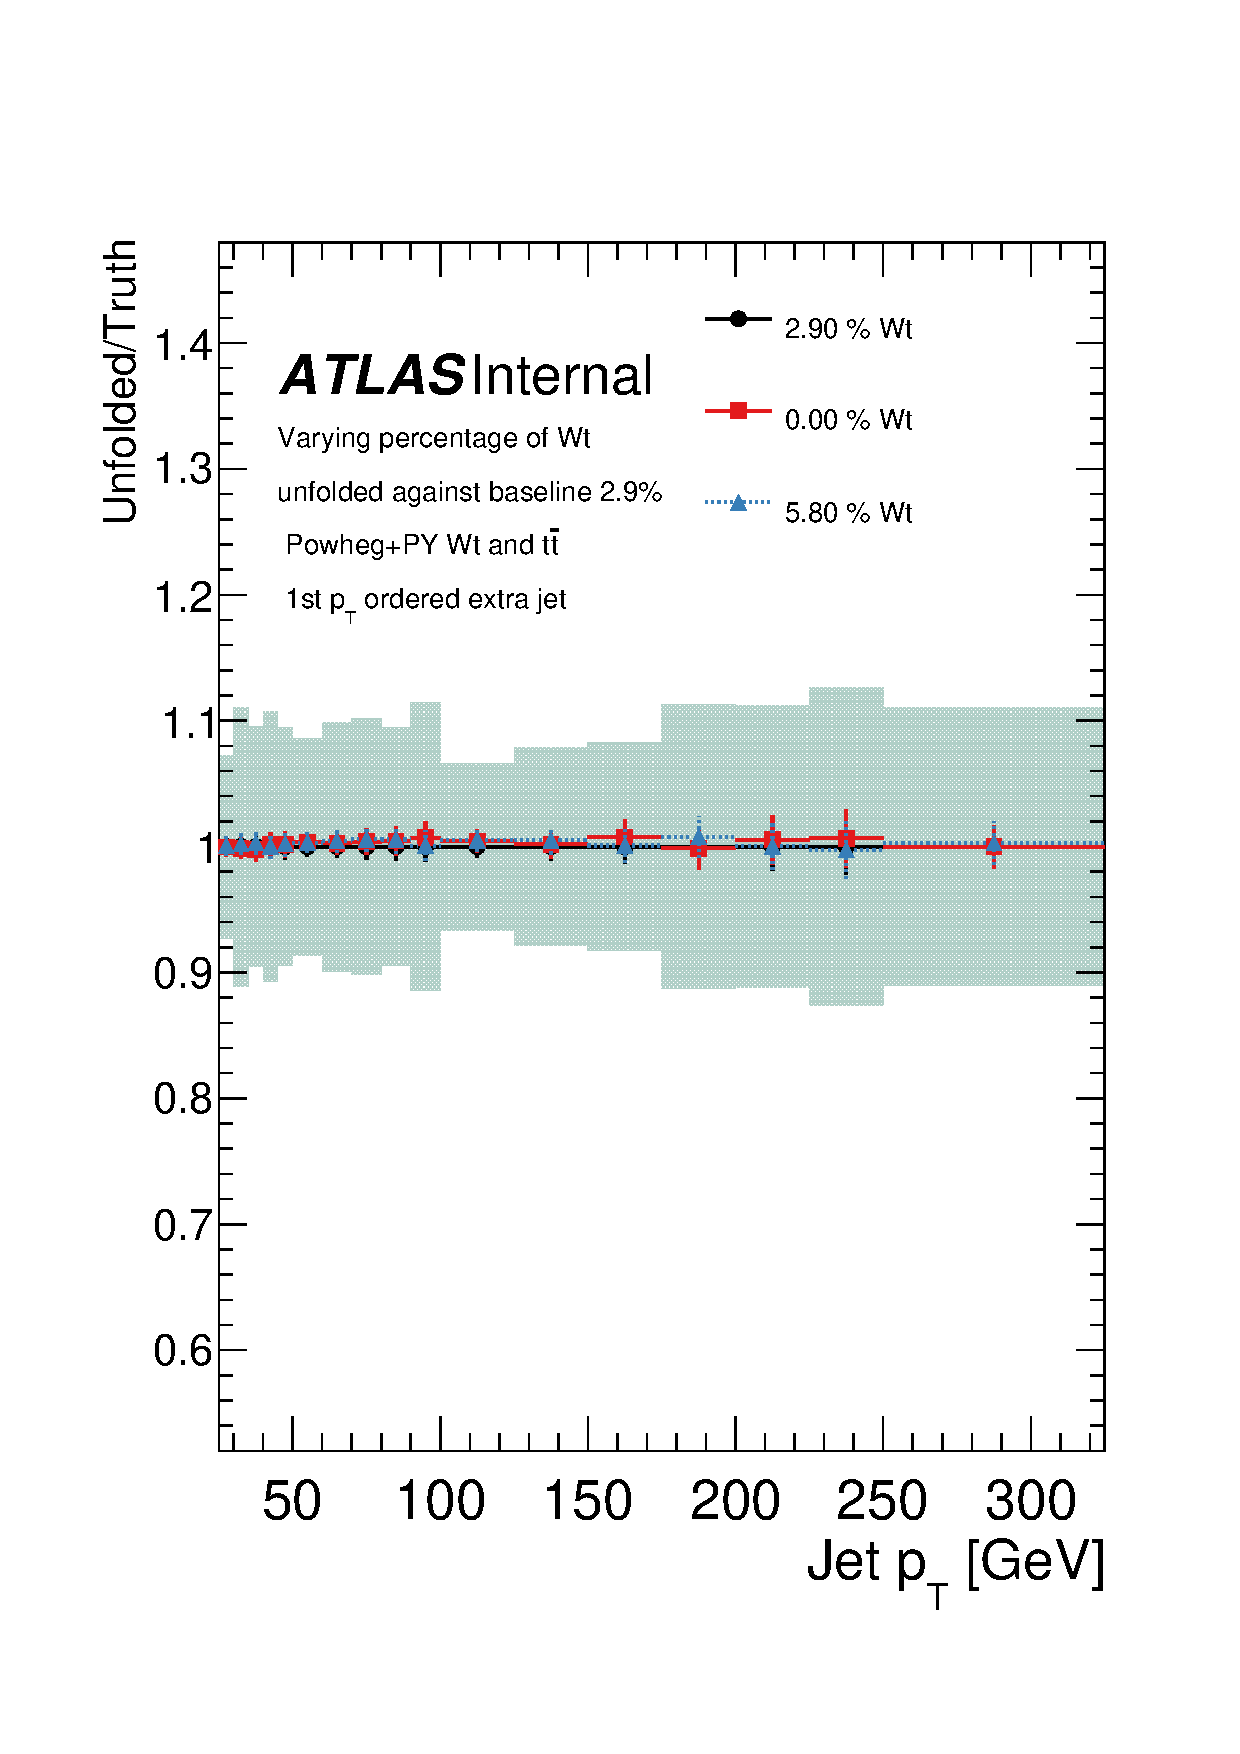
\includegraphics[width=\textwidth]{fig/Wt/TruthRatioJet0.pdf}
\end{subfigure}
~
\begin{subfigure}[]{0.3\textwidth}
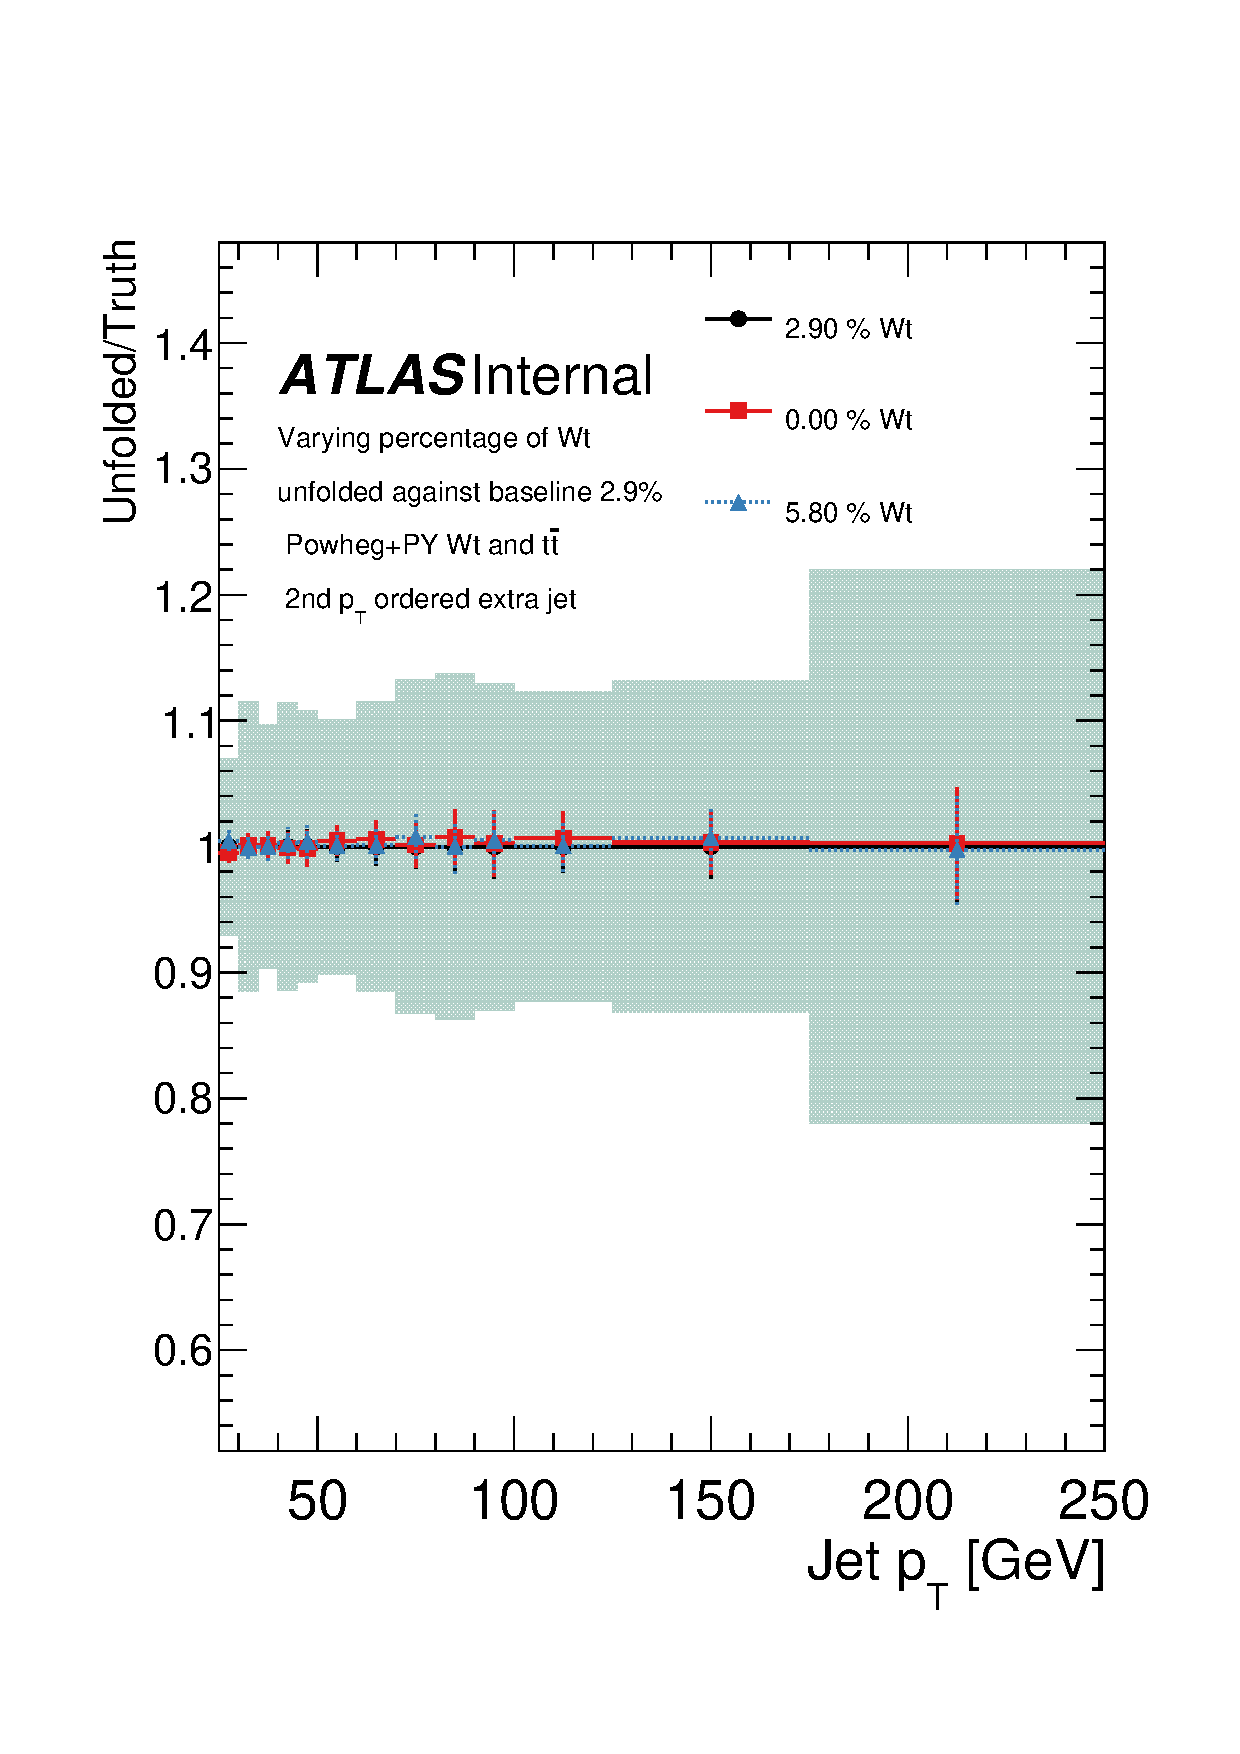
\includegraphics[width=\textwidth]{fig/Wt/TruthRatioJet1.pdf}
\end{subfigure}
~
\begin{subfigure}[]{0.3\textwidth}
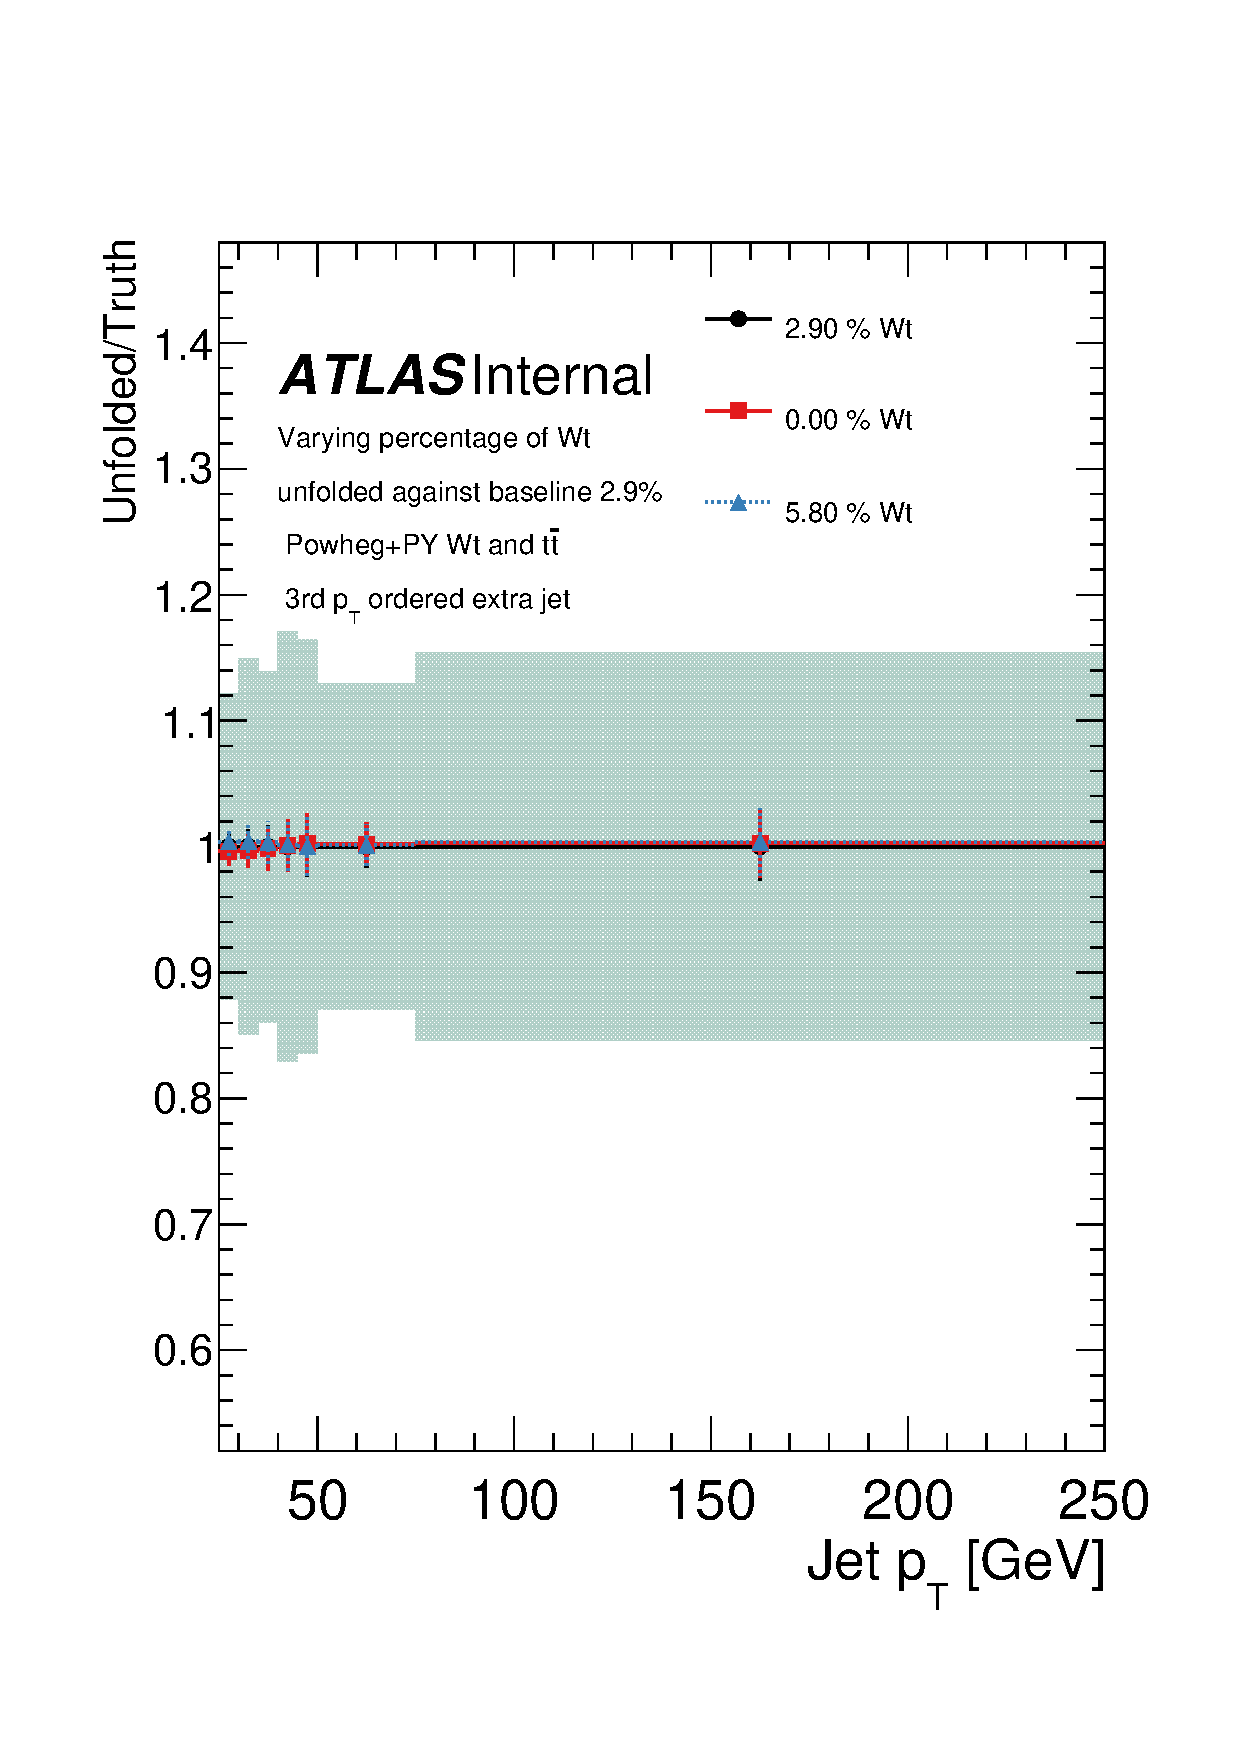
\includegraphics[width=\textwidth]{fig/Wt/TruthRatioJet2.pdf}
\end{subfigure}
~
\begin{subfigure}[]{0.3\textwidth}
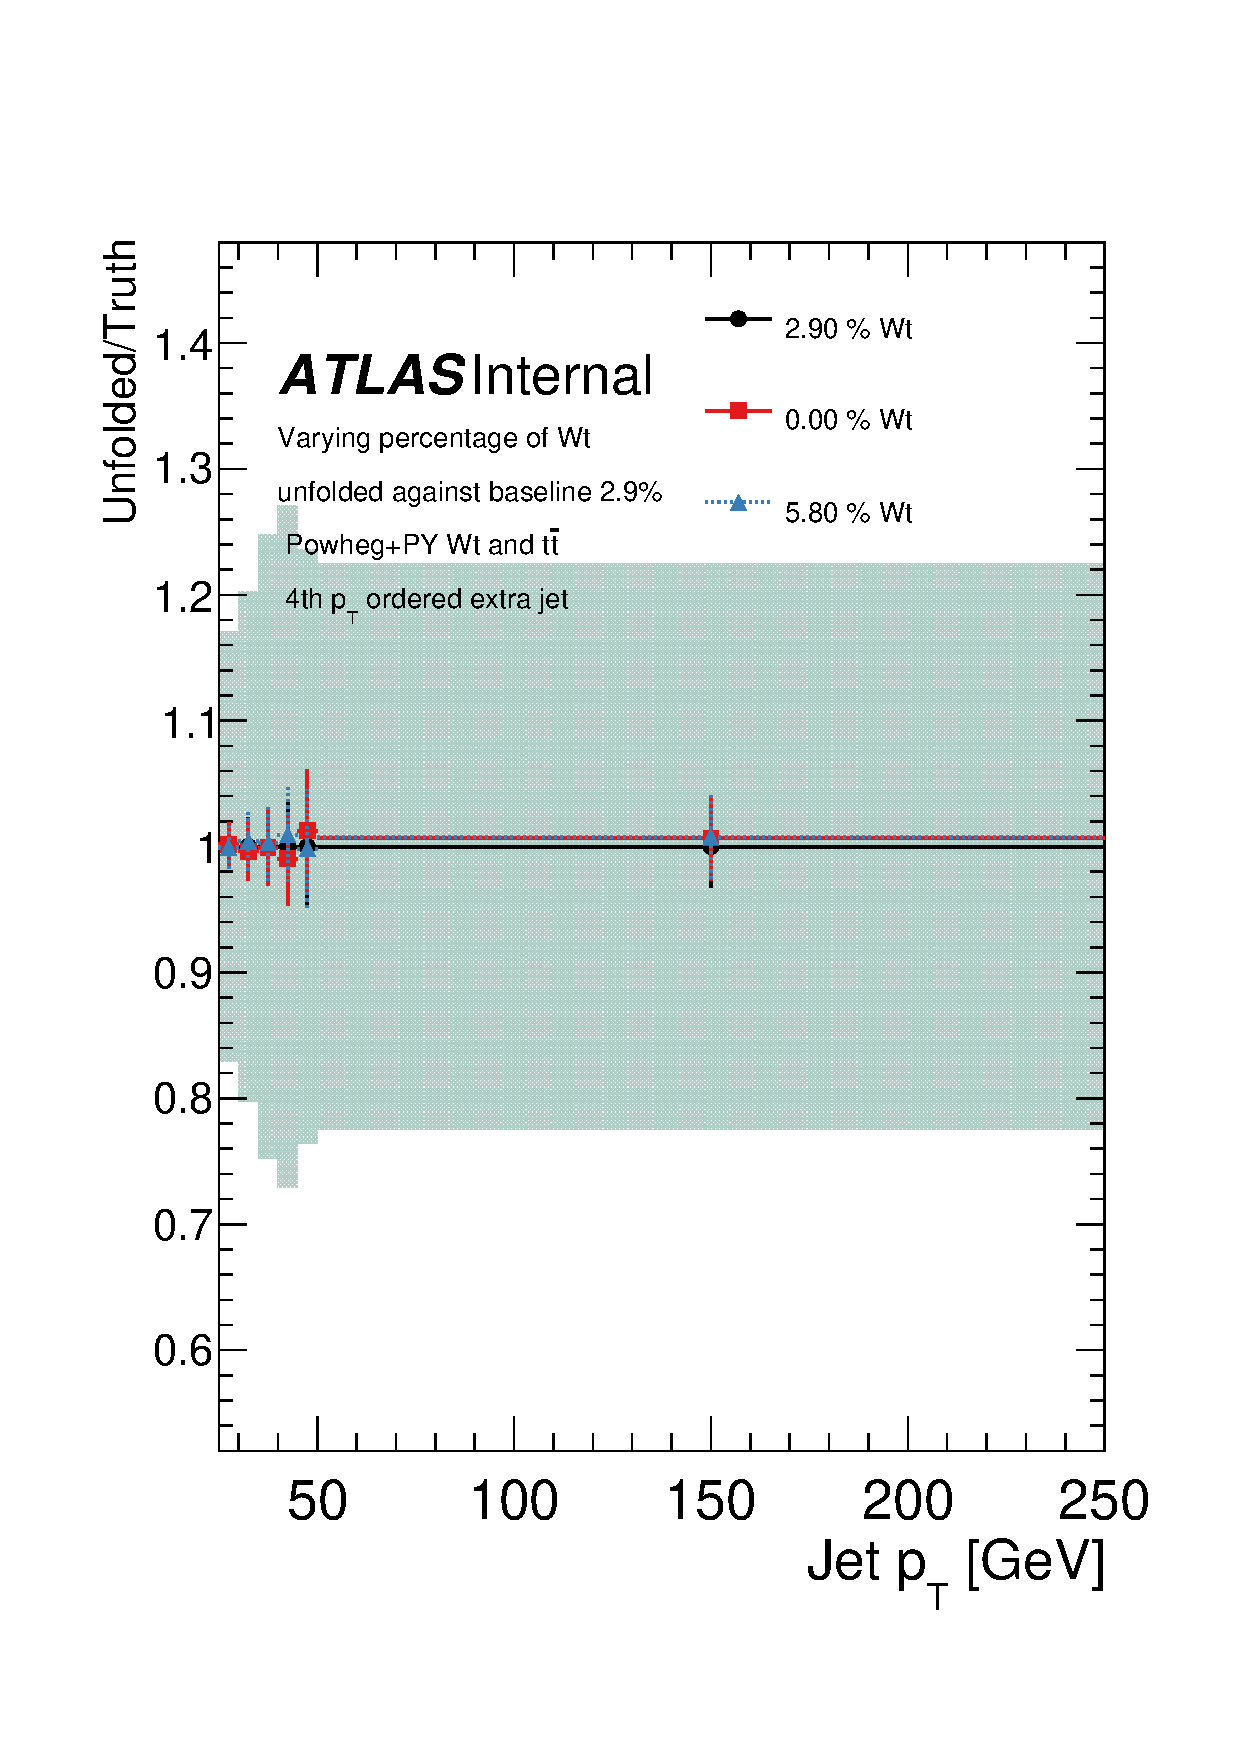
\includegraphics[width=\textwidth]{fig/Wt/TruthRatioJet3.pdf}
\end{subfigure}
~
\begin{subfigure}[]{0.3\textwidth}
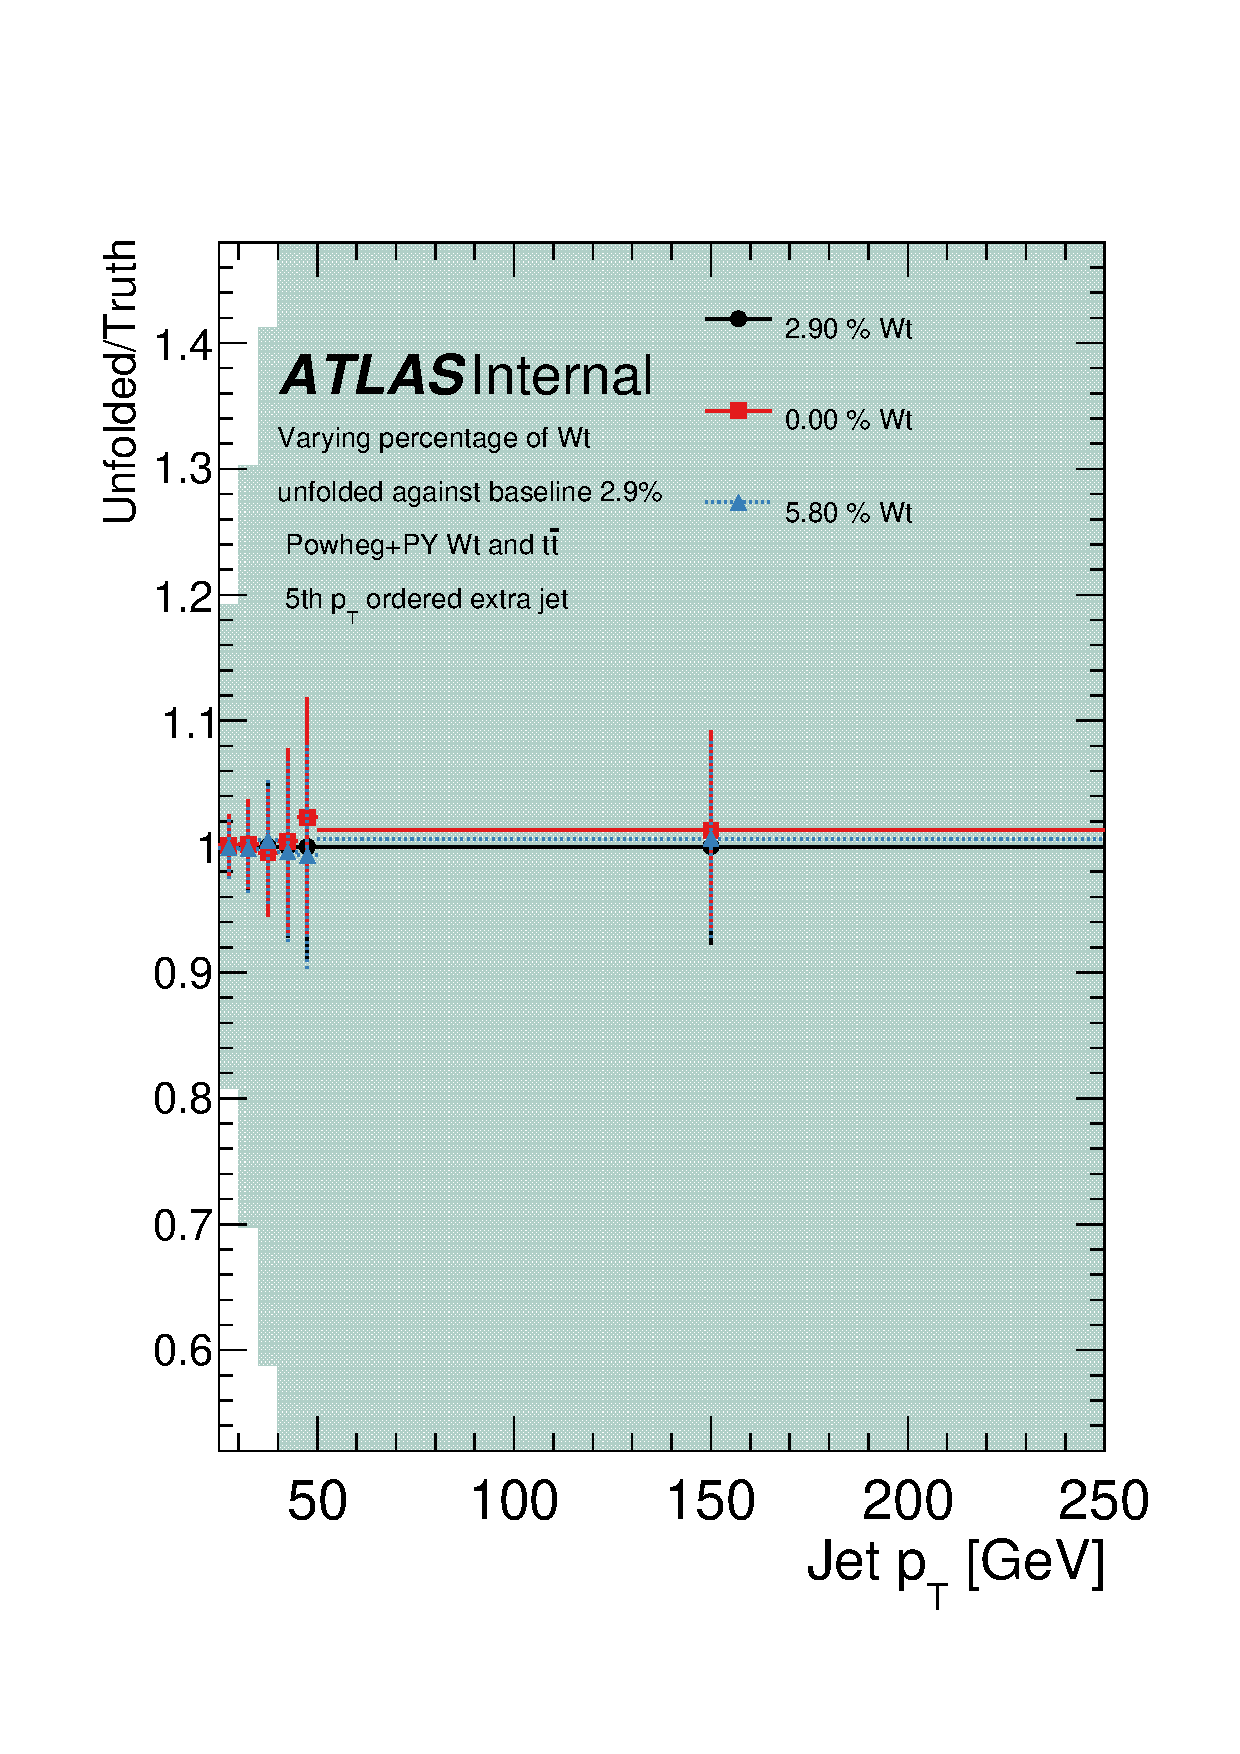
\includegraphics[width=\textwidth]{fig/Wt/TruthRatioJet4.pdf}
\end{subfigure}
~
\caption{The systematic uncertainty on the unfolded spectrum due uncertainties in the
Wt
atio of $N^{\textrm{unfolded}}$ over $N^{\textrm{true}}$ jets per \GeV for events from \ttbar+single top simulation. The response matrix is filled with the 97.1\% \ttbar events and nominal 2.9\% single top events. The rate of single top is then varied and unfolded against the nominal matrix.}
\label{fig:WtRat}
\end{figure}
\clearpage
